\documentclass[10pt]{article}

\usepackage[a4paper,margin=3cm]{geometry}
\usepackage{amsmath,amsfonts,amsthm,bm}
\usepackage{amssymb}
\usepackage{afterpage}
\usepackage{lastpage}
\usepackage{graphicx}
\usepackage{fancyhdr}
\usepackage{multirow}
\usepackage{hhline}
\usepackage{titlesec}
\usepackage{enumitem}
\usepackage{mathtools}
\usepackage{indentfirst}
\usepackage{bbm}
\usepackage{float}
\usepackage[affil-it]{authblk}

\titleformat{\section}
 {\normalfont\fontsize{16}{19}\selectfont}{\thesection.}{1em}{}
\titleformat{\subsection}
 {\normalfont\fontsize{14}{17}\selectfont}{\thesubsection}{1em}{}
\titleformat{\subsubsection}
 {\normalfont\fontsize{14}{17}\selectfont}{\thesubsubsection}{1em}{}
\pagestyle{fancy}
\fancyhead{}
\fancyfoot{}
\renewcommand{\headrulewidth}{0pt}
\renewcommand{\refname}{\vskip -1cm}
\fancyfoot[R]{p. \thepage\ / \pageref{LastPage}}

\numberwithin{equation}{section}
\restylefloat{table}


\DeclareMathOperator*{\minimize}{minimize\;\;}
\DeclareMathOperator*{\subject_to}{subject\;to\;\;}
\DeclareMathOperator{\asinh}{asinh}
\DeclareMathOperator{\sgn}{sgn}


\begin{document}
\section{Project Setup}
\begin{enumerate}
    \item Project Title: A Tiny World: Atom Simulation/Rendering
    \item Members and Roles:
        \subitem Chung An, Chen (Andy), 5120AG05-1
            \subsubitem Software Development, Final Report, Team Management
        \subitem Yang, Liu, 5121FG59
            \subsubitem Software Development, Setting Up Demo, Slides
        \subitem LinXi, Tao, 5121FG25
            \subsubitem Material Research, Slides, Final Report
    \item Project Timeline:
        \subitem 12/12 - 12/15 Project Initiation (Done)
            \subsubitem Decided to go with an Atom Simulation/Rendering
            \subsubitem Backup option: Fluid simulations
        \subitem 12/15 - 12/18 Project Development Tool Investigation (Done) 
            \subsubitem Decided to use \textbf{Taichi}, a Domain-specific-language (DSL) written in Python and C++ for graphical simulations, as our main development tool
        \subitem 12/18 - 12/24 Tinkering and Experimenting with \textbf{Taichi} and Finalizing Our Initial Report
        \subitem 12/24 - 1/01 Creating Several Prototypes
        \subitem 1/01 - 1/14 Finalizing the Prototype and Refining It
        \subitem 1/14 - 1/17 Setting Up a Demo Server/Host
        \subitem 1/17 - 1/31 Creating Slides for the Presentation and Putting together Our Final Report
\end{enumerate}
\section{Project Description}
    This project aims to simulate and render an atom's presence in a three-dimensional space. The simulation will be grounded on the more accurate electron cloud model, shown in Figure 1 belown. An electron cloud model depicts the occurence of an atom's electrons by a density map containing numerous sparse dots. In any region, the density of the dots draws a directly proportional relationship to the probability of an electron being present. To make this feasible, We leverage a recently-built parallel programming language, namely \textbf{Taichi}, as our main development framework.

\begin{figure}[H]
\centering
  \begin{minipage}[b]{0.4\textwidth}
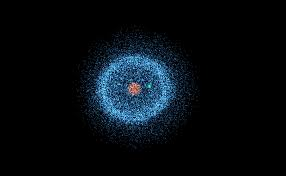
\includegraphics[width=\textwidth]{./concept_1.jpeg}
  \end{minipage}
    \begin{minipage}[b]{0.4\textwidth}
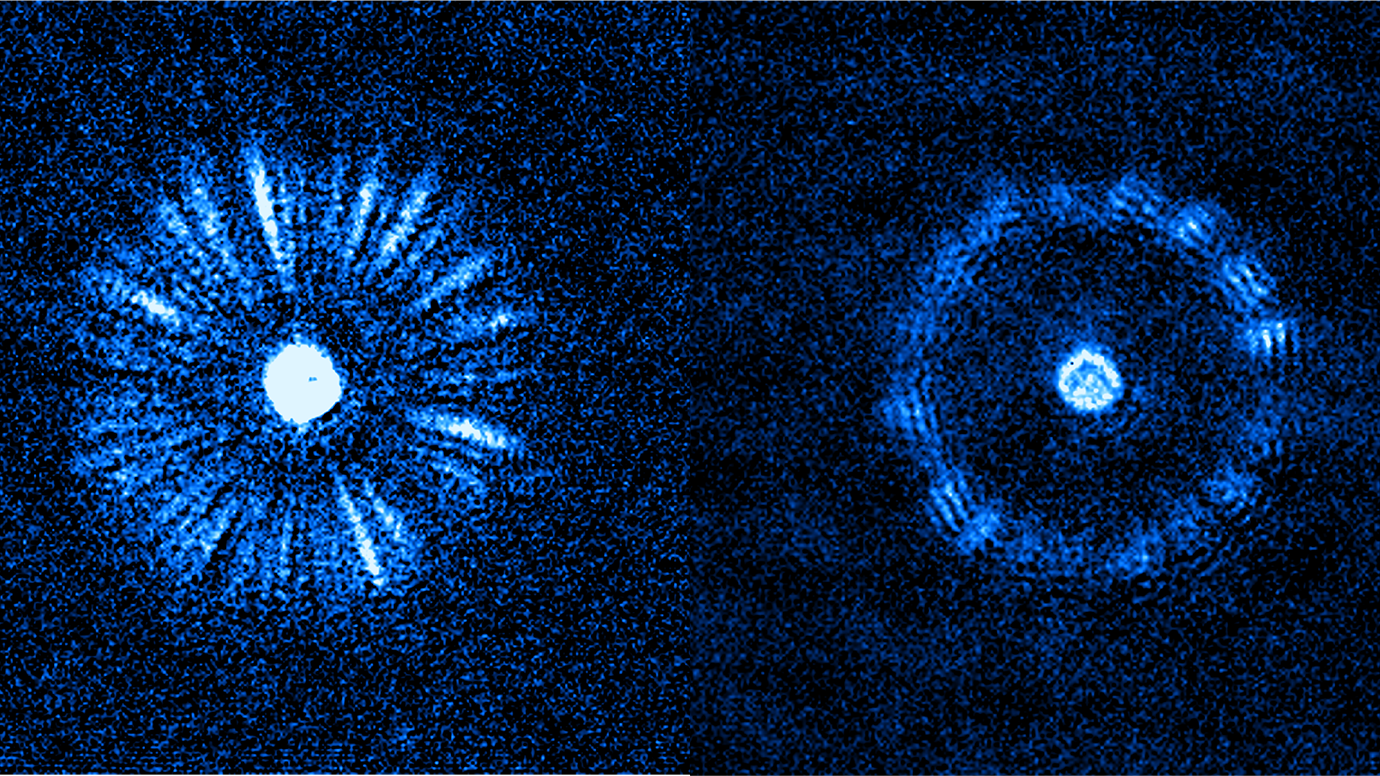
\includegraphics[width=\textwidth]{./concept_2.png}
  \end{minipage}
 \caption{Atoms and Their Nucleus and Electron Cloud}\label{fig1} 
\label{fig1}
\end{figure}

\end{document}
